% Created by tikzDevice version 0.8.1 on 2015-07-23 00:07:06
% !TEX encoding = UTF-8 Unicode
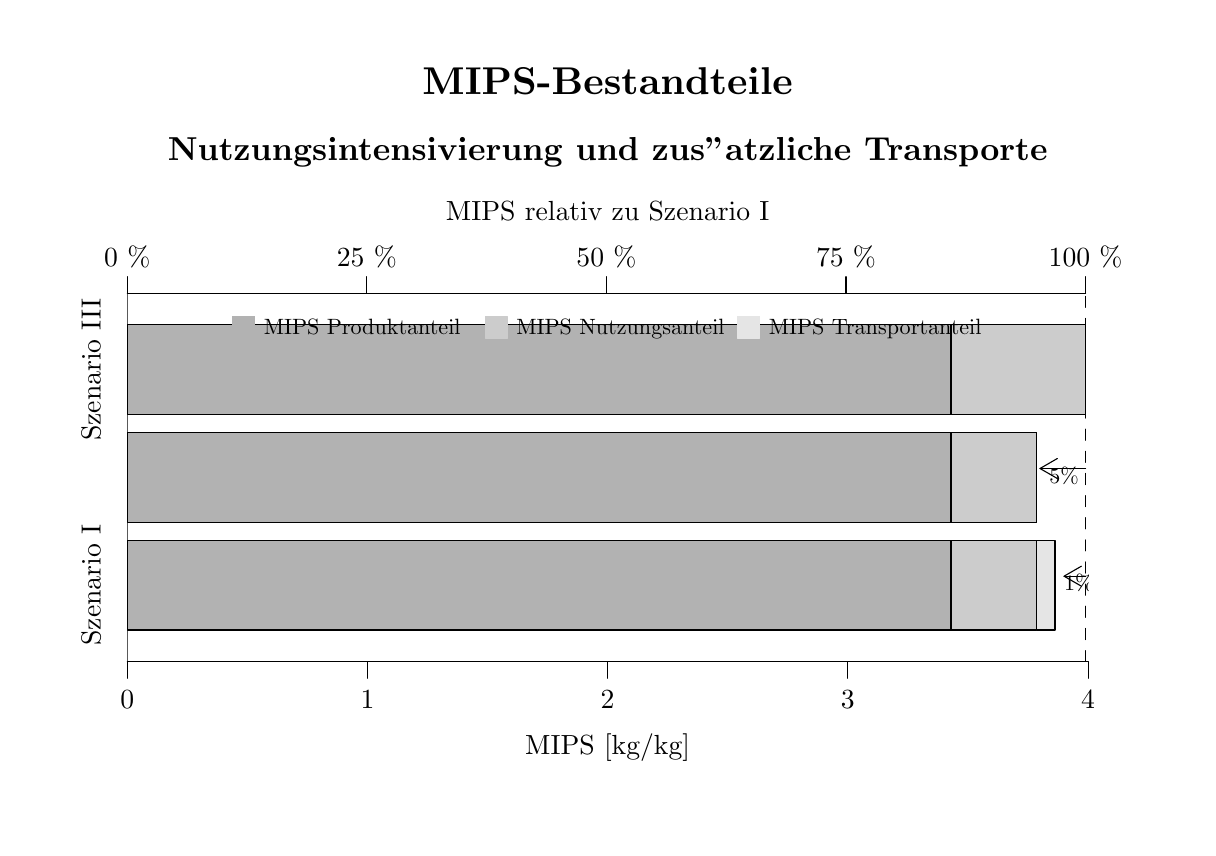
\begin{tikzpicture}[x=1pt,y=1pt]
\definecolor{fillColor}{RGB}{255,255,255}
\path[use as bounding box,fill=fillColor,fill opacity=0.00] (0,0) rectangle (419.17,289.08);
\begin{scope}
\path[clip] (  0.00,  0.00) rectangle (419.17,289.08);
\definecolor{drawColor}{RGB}{0,0,0}
\definecolor{fillColor}{gray}{0.70}

\path[draw=drawColor,line width= 0.4pt,line join=round,line cap=round,fill=fillColor] ( 36.00, 71.41) rectangle (333.63,103.84);
\definecolor{fillColor}{gray}{0.80}

\path[draw=drawColor,line width= 0.4pt,line join=round,line cap=round,fill=fillColor] (333.63, 71.41) rectangle (364.57,103.84);
\definecolor{fillColor}{gray}{0.90}

\path[draw=drawColor,line width= 0.4pt,line join=round,line cap=round,fill=fillColor] (364.57, 71.41) rectangle (371.20,103.84);
\definecolor{fillColor}{gray}{0.70}

\path[draw=drawColor,line width= 0.4pt,line join=round,line cap=round,fill=fillColor] ( 36.00,110.33) rectangle (333.63,142.75);
\definecolor{fillColor}{gray}{0.80}

\path[draw=drawColor,line width= 0.4pt,line join=round,line cap=round,fill=fillColor] (333.63,110.33) rectangle (364.57,142.75);
\definecolor{fillColor}{gray}{0.90}

\path[draw=drawColor,line width= 0.4pt,line join=round,line cap=round,fill=fillColor] (364.57,110.33) rectangle (364.57,142.75);
\definecolor{fillColor}{gray}{0.70}

\path[draw=drawColor,line width= 0.4pt,line join=round,line cap=round,fill=fillColor] ( 36.00,149.24) rectangle (333.63,181.67);
\definecolor{fillColor}{gray}{0.80}

\path[draw=drawColor,line width= 0.4pt,line join=round,line cap=round,fill=fillColor] (333.63,149.24) rectangle (382.28,181.67);
\definecolor{fillColor}{gray}{0.90}

\path[draw=drawColor,line width= 0.4pt,line join=round,line cap=round,fill=fillColor] (382.28,149.24) rectangle (382.28,181.67);
\end{scope}
\begin{scope}
\path[clip] (  0.00,  0.00) rectangle (419.17,289.08);
\definecolor{drawColor}{RGB}{0,0,0}

\node[text=drawColor,rotate= 90.00,anchor=base,inner sep=0pt, outer sep=0pt, scale=  1.00] at ( 26.40, 87.63) {Szenario I};

\node[text=drawColor,rotate= 90.00,anchor=base,inner sep=0pt, outer sep=0pt, scale=  1.00] at ( 26.40,165.45) {Szenario III};

\path[draw=drawColor,line width= 0.4pt,line join=round,line cap=round] ( 36.00,193.08) -- (382.28,193.08);

\path[draw=drawColor,line width= 0.4pt,line join=round,line cap=round] ( 36.00,193.08) -- ( 36.00,199.08);

\path[draw=drawColor,line width= 0.4pt,line join=round,line cap=round] (122.57,193.08) -- (122.57,199.08);

\path[draw=drawColor,line width= 0.4pt,line join=round,line cap=round] (209.14,193.08) -- (209.14,199.08);

\path[draw=drawColor,line width= 0.4pt,line join=round,line cap=round] (295.71,193.08) -- (295.71,199.08);

\path[draw=drawColor,line width= 0.4pt,line join=round,line cap=round] (382.28,193.08) -- (382.28,199.08);

\node[text=drawColor,anchor=base,inner sep=0pt, outer sep=0pt, scale=  1.00] at ( 36.00,202.68) {0 \%};

\node[text=drawColor,anchor=base,inner sep=0pt, outer sep=0pt, scale=  1.00] at (122.57,202.68) {25 \%};

\node[text=drawColor,anchor=base,inner sep=0pt, outer sep=0pt, scale=  1.00] at (209.14,202.68) {50 \%};

\node[text=drawColor,anchor=base,inner sep=0pt, outer sep=0pt, scale=  1.00] at (295.71,202.68) {75 \%};

\node[text=drawColor,anchor=base,inner sep=0pt, outer sep=0pt, scale=  1.00] at (382.28,202.68) {100 \%};

\node[text=drawColor,anchor=base,inner sep=0pt, outer sep=0pt, scale=  1.00] at (209.58,219.48) {MIPS relativ zu Szenario I};

\path[draw=drawColor,line width= 0.4pt,line join=round,line cap=round] ( 36.00, 60.00) -- (383.17, 60.00);

\path[draw=drawColor,line width= 0.4pt,line join=round,line cap=round] ( 36.00, 60.00) -- ( 36.00, 54.00);

\path[draw=drawColor,line width= 0.4pt,line join=round,line cap=round] (122.79, 60.00) -- (122.79, 54.00);

\path[draw=drawColor,line width= 0.4pt,line join=round,line cap=round] (209.58, 60.00) -- (209.58, 54.00);

\path[draw=drawColor,line width= 0.4pt,line join=round,line cap=round] (296.37, 60.00) -- (296.37, 54.00);

\path[draw=drawColor,line width= 0.4pt,line join=round,line cap=round] (383.17, 60.00) -- (383.17, 54.00);

\node[text=drawColor,anchor=base,inner sep=0pt, outer sep=0pt, scale=  1.00] at ( 36.00, 43.20) {0};

\node[text=drawColor,anchor=base,inner sep=0pt, outer sep=0pt, scale=  1.00] at (122.79, 43.20) {1};

\node[text=drawColor,anchor=base,inner sep=0pt, outer sep=0pt, scale=  1.00] at (209.58, 43.20) {2};

\node[text=drawColor,anchor=base,inner sep=0pt, outer sep=0pt, scale=  1.00] at (296.37, 43.20) {3};

\node[text=drawColor,anchor=base,inner sep=0pt, outer sep=0pt, scale=  1.00] at (383.17, 43.20) {4};

\node[text=drawColor,anchor=base,inner sep=0pt, outer sep=0pt, scale=  1.00] at (209.58, 26.40) {MIPS [kg/kg]};
\end{scope}
\begin{scope}
\path[clip] ( 36.00, 60.00) rectangle (383.17,193.08);
\definecolor{drawColor}{RGB}{0,0,0}

\path[draw=drawColor,line width= 0.4pt,line join=round,line cap=round] ( 36.00, 60.00) -- ( 36.00,193.08);

\path[draw=drawColor,line width= 0.4pt,dash pattern=on 4pt off 4pt ,line join=round,line cap=round] (382.28, 60.00) -- (382.28,193.08);
\definecolor{drawColor}{gray}{0.70}
\definecolor{fillColor}{gray}{0.70}

\path[draw=drawColor,line width= 0.4pt,line join=round,line cap=round,fill=fillColor] ( 74.12,176.83) rectangle ( 82.10,184.81);
\definecolor{drawColor}{gray}{0.80}
\definecolor{fillColor}{gray}{0.80}

\path[draw=drawColor,line width= 0.4pt,line join=round,line cap=round,fill=fillColor] (165.37,176.83) rectangle (173.35,184.81);
\definecolor{drawColor}{gray}{0.90}
\definecolor{fillColor}{gray}{0.90}

\path[draw=drawColor,line width= 0.4pt,line join=round,line cap=round,fill=fillColor] (256.62,176.83) rectangle (264.60,184.81);
\definecolor{drawColor}{RGB}{0,0,0}

\node[text=drawColor,anchor=base west,inner sep=0pt, outer sep=0pt, scale=  0.80] at ( 85.31,178.06) {MIPS Produktanteil      };

\node[text=drawColor,anchor=base west,inner sep=0pt, outer sep=0pt, scale=  0.80] at (176.56,178.06) {MIPS Nutzungsanteil      };

\node[text=drawColor,anchor=base west,inner sep=0pt, outer sep=0pt, scale=  0.80] at (267.81,178.06) {MIPS Transportanteil};
\end{scope}
\begin{scope}
\path[clip] (  0.00,  0.00) rectangle (419.17,289.08);
\definecolor{drawColor}{RGB}{0,0,0}

\node[text=drawColor,anchor=base,inner sep=0pt, outer sep=0pt, scale=  1.40] at (209.58,265.08) {\bfseries MIPS-Bestandteile};

\node[text=drawColor,anchor=base,inner sep=0pt, outer sep=0pt, scale=  1.20] at (209.58,241.08) {\bfseries Nutzungsintensivierung und zus"atzliche Transporte};
\end{scope}
\begin{scope}
\path[clip] ( 36.00, 60.00) rectangle (383.17,193.08);
\definecolor{drawColor}{RGB}{0,0,0}

\node[text=drawColor,anchor=base west,inner sep=0pt, outer sep=0pt, scale=  0.80] at (374.49, 85.63) {1\%};

\path[draw=drawColor,line width= 0.4pt,line join=round,line cap=round] (374.49, 90.87) -- (382.30, 90.87);

\path[draw=drawColor,line width= 0.4pt,line join=round,line cap=round] (380.75, 94.48) --
	(374.49, 90.87) --
	(380.75, 87.26);

\node[text=drawColor,anchor=base,inner sep=0pt, outer sep=0pt, scale=  0.80] at (374.49,124.54) {5\%};

\path[draw=drawColor,line width= 0.4pt,line join=round,line cap=round] (365.81,129.78) -- (382.30,129.78);

\path[draw=drawColor,line width= 0.4pt,line join=round,line cap=round] (372.07,133.40) --
	(365.81,129.78) --
	(372.07,126.17);
\end{scope}
\end{tikzpicture}
